\documentclass[11pt]{standalone}
\usepackage{amssymb}
\usepackage{amsmath}
\usepackage[no-math]{fontspec}
\usepackage{unicode-math}
\usepackage{libertinus}
\usepackage{pgf,xcolor}
\usepackage{tikz}
\usetikzlibrary{arrows.meta, backgrounds}
\usepackage{pgfplots}
\pgfplotsset{compat=newest}

\setmainfont{Libertinus Serif}
\setmathfont{Libertinus Math}

\definecolor{my_darkgray}{HTML}{484949}
\definecolor{my_lightgray}{HTML}{F3F4F4}
\definecolor{my_darkblue}{HTML}{005A94}
\definecolor{my_lightblue}{HTML}{CCDEE9}
\definecolor{my_yellow}{HTML}{FFEC7F}
\definecolor{my_red}{HTML}{E60000}
\definecolor{my_orange}{HTML}{E87846}

\begin{document}

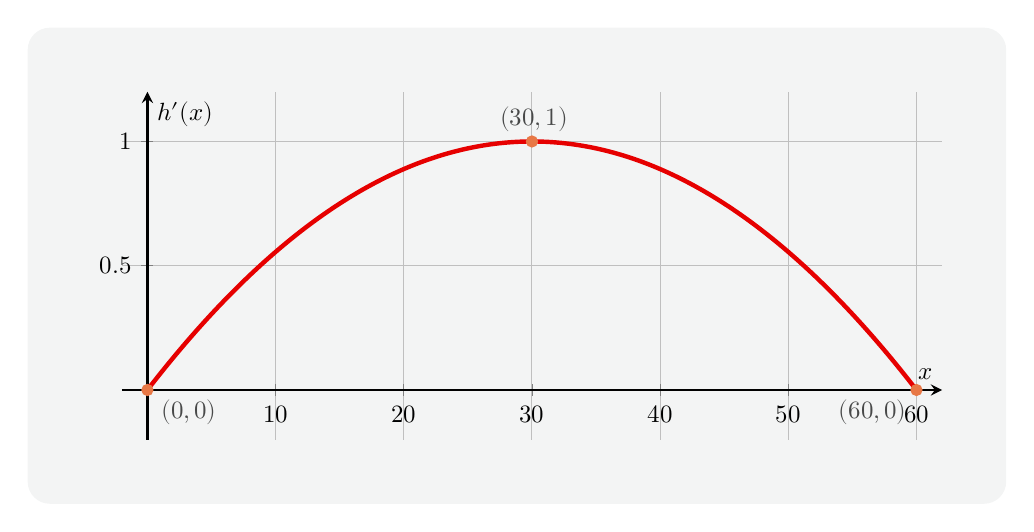
\begin{tikzpicture}[
    show background rectangle,
    background rectangle/.style={fill=my_lightgray, rounded corners=8pt},
    inner frame sep=0.8cm
]

\begin{axis}[
    width=12cm,
    height=6cm,
    axis lines = center,
    xlabel = {$x$},
    ylabel = {$h'(x)$},
    xmin=-2, xmax=62,
    ymin=-0.2, ymax=1.2,
    grid = both,
    % Omit axis equal here so that the curve is clearly visible
    axis line style={thick},
    ticklabel style={font=\small},
    label style={font=\small},
]

% slope function h'(x) = x/15 - x^2/900 on [0, 60]
\addplot[
    draw=my_red,
    ultra thick,
    samples=300,
    domain=0:60
]
{0.0666666667*x - 0.00111111111*x^2};

% mark the base (0, 0)
\addplot[
    only marks,
    mark=*,
    mark size=2pt,
    draw=my_orange,
    fill=my_orange
]
coordinates {(0,0)};

\node[anchor=north west, font=\small, my_darkgray]
at (axis cs:0,0) {$\,(0, 0)$};

% mark the summit (60, 0)
\addplot[
    only marks,
    mark=*,
    mark size=2pt,
    draw=my_orange,
    fill=my_orange
]
coordinates {(60,0)};

\node[anchor=north east, font=\small, my_darkgray]
at (axis cs:60,0) {$(60, 0)$};

% mark the maximum slope at (30, 1)
\addplot[
    only marks,
    mark=*,
    mark size=2pt,
    draw=my_orange,
    fill=my_orange
]
coordinates {(30,1)};

\node[anchor=south, font=\small, my_darkgray]
at (axis cs:30,1) {$\,(30, 1)$};

\node[anchor=south west, font=\small\bfseries, my_darkgray]
at (rel axis cs:0.02,0.98)
{Slope function $h'(x) = \dfrac{x}{15} - \dfrac{x^2}{900}$};

\end{axis}

\end{tikzpicture}

\end{document}